\documentclass[conference]{IEEEtran}
\usepackage[utf8]{inputenc}
\usepackage{graphicx}
\usepackage{hyperref}
\usepackage{listings}
\usepackage{amsmath}
\usepackage{url}

\title{WebScrepStatusQlik: Monitoramento Automatizado de Tarefas do Qlik Sense com Envio de Alertas via WhatsApp}
\author{\IEEEauthorblockN{Wagner Filho}
\IEEEauthorblockA{Instituto de Pós-Graduação \\ Universidade Federal de Goiás \\ wagner.filho@example.com}}

\begin{document}
\maketitle

\begin{abstract}
Este artigo apresenta o sistema WebScrepStatusQlik, uma solução de coleta, transformação e notificação automática de falhas de execução em tarefas do Qlik Sense. A solução integra componentes de scraping dinâmico com Selenium, tratamento e padronização de dados, geração de relatórios e envio automatizado via EvolutionAPI para WhatsApp. O trabalho aborda os aspectos técnicos, éticos e legais envolvidos no uso de dados automatizados e apresenta diretrizes de reprodutibilidade.
\end{abstract}

\section{Introdução e Motivação}
A análise de dados em larga escala, especialmente em plataformas como Qlik Sense, depende da execução contínua e sem falhas de tarefas automatizadas. A ausência de mecanismos robustos de notificação sobre falhas críticas motiva o desenvolvimento de ferramentas auxiliares como o WebScrepStatusQlik, que visa automatizar a coleta de status de tarefas, geração de relatórios e envio de alertas.

\section{Fundamentação Teórica}
A automação de coleta de dados via \textit{web scraping} é tema amplamente explorado em projetos acadêmicos e industriais \cite{mitchell2018web}. Frameworks como Selenium, BeautifulSoup e Scrapy são referência nesse campo. Além disso, práticas de engenharia de dados orientadas a camadas (raw, clean, analytics) vêm sendo consolidadas em arquiteturas modernas \cite{bonomi2015data}. APIs de mensagens como o WhatsApp Business API vêm sendo exploradas para automações em tempo real.

\section{Método}
\subsection{Problema e Importância}
Falta um mecanismo nativo no Qlik Sense para envio proativo de alertas detalhados sobre falhas, o que compromete a confiabilidade de sistemas analíticos. Este projeto visa preencher essa lacuna com uma abordagem leve, modular e automatizada.

\subsection{Arquitetura do Pipeline}
O sistema adota um pipeline de três camadas:
\begin{itemize}
  \item \textbf{Extração}: via Selenium, realizando scraping de páginas HTML dinâmicas da interface do Qlik Sense (QMC e NPrinting).
  \item \textbf{Engenharia de Dados}: separação dos dados em camadas \texttt{raw} (logs originais) e \texttt{clean} (dados padronizados e filtrados), com transformações reproduzíveis.
  \item \textbf{Análise e Entrega}: geração de relatórios em HTML + PDF via Jinja2/pdfkit e envio via EvolutionAPI.
\end{itemize}

\subsection{Reprodutibilidade e Documentação}
O projeto inclui README detalhado com instruções de instalação, uso e replicação. Scripts e dependências estão organizados por função. Todas as transformações são reproduzíveis.

\section{Resultados e Discussões}
O sistema foi testado com sucesso em ambiente Windows com Qlik Sense local. Resultados obtidos:
\begin{itemize}
  \item Coleta contínua dos status de execução das tarefas do QMC.
  \item Identificação e armazenamento dos logs de falha do NPrinting.
  \item Geração de relatórios organizados por status e data.
  \item Envio automatizado dos relatórios via WhatsApp, tanto para indivíduos quanto grupos.
\end{itemize}

\begin{figure}[ht]
\centering
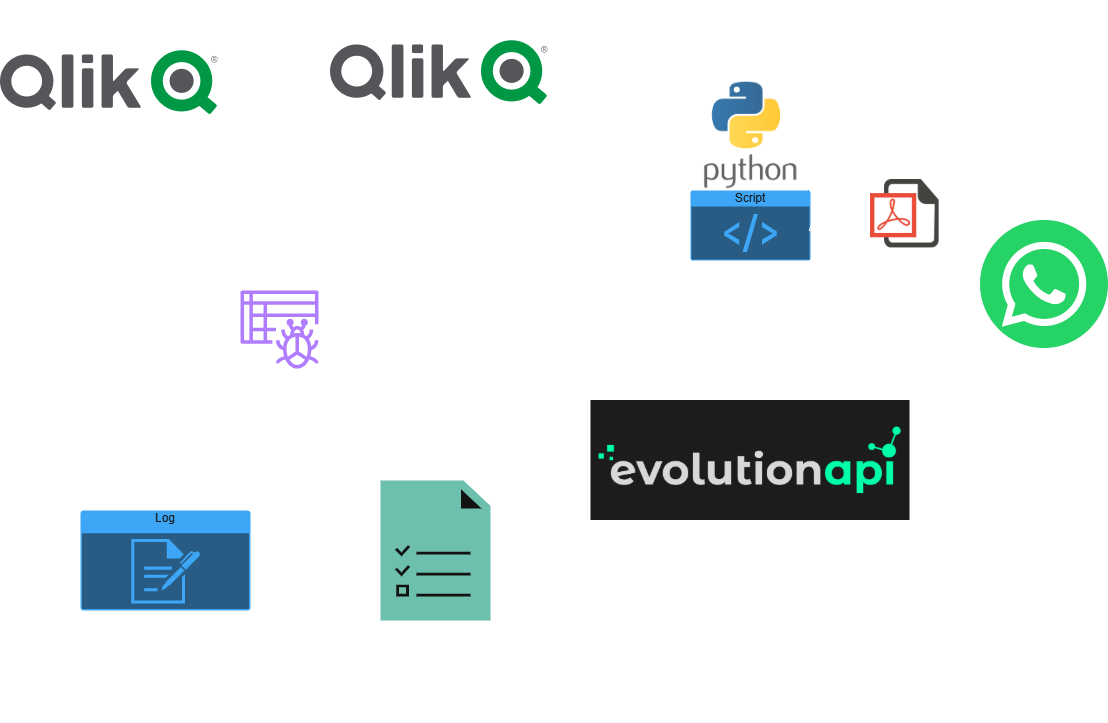
\includegraphics[width=0.45\textwidth]{img/WebScrep_QMC.drawio.png}
\caption{Arquitetura do pipeline WebScrepStatusQlik}
\end{figure}

\section{Reflexões Éticas e Limitações}
A coleta respeita \texttt{robots.txt} do ambiente Qlik local. Dados pessoais não são processados. O uso da EvolutionAPI respeita os termos da plataforma. A LGPD foi considerada, e não há coleta identificável de indivíduos. Limitações incluem dependência da interface gráfica e ausência de fallback para falhas na própria API do WhatsApp.

\section{Conclusão e Trabalhos Futuros}
O WebScrepStatusQlik mostrou-se eficaz e reprodutível. Pretende-se como trabalho futuro:
\begin{itemize}
  \item Implementar versão dockerizada e compatível com servidores Linux.
  \item Integrar com ferramentas de monitoramento como Grafana ou Zabbix.
  \item Adicionar painel de controle web para parametrização e auditoria.
\end{itemize}

\section*{Licenças e Fontes Utilizadas}
\begin{itemize}
  \item Qlik Sense – Licença corporativa.
  \item EvolutionAPI – Licença de uso próprio, conforme \url{https://evolution-api.com/terms}.
  \item ChromeDriver – Licenciado pelo Google sob BSD.
  \item Dados armazenados localmente, sem uso de bases públicas externas.
\end{itemize}

\bibliographystyle{IEEEtran}
\bibliography{referencias}

\end{document}
